\documentclass[1p]{elsarticle_modified}
%\bibliographystyle{elsarticle-num}

%\usepackage[colorlinks]{hyperref}
%\usepackage{abbrmath_seonhwa} %\Abb, \Ascr, \Acal ,\Abf, \Afrak
\usepackage{amsfonts}
\usepackage{amssymb}
\usepackage{amsmath}
\usepackage{amsthm}
\usepackage{scalefnt}
\usepackage{amsbsy}
\usepackage{kotex}
\usepackage{caption}
\usepackage{subfig}
\usepackage{color}
\usepackage{graphicx}
\usepackage{xcolor} %% white, black, red, green, blue, cyan, magenta, yellow
\usepackage{float}
\usepackage{setspace}
\usepackage{hyperref}

\usepackage{tikz}
\usetikzlibrary{arrows}

\usepackage{multirow}
\usepackage{array} % fixed length table
\usepackage{hhline}

%%%%%%%%%%%%%%%%%%%%%
\makeatletter
\renewcommand*\env@matrix[1][\arraystretch]{%
	\edef\arraystretch{#1}%
	\hskip -\arraycolsep
	\let\@ifnextchar\new@ifnextchar
	\array{*\c@MaxMatrixCols c}}
\makeatother %https://tex.stackexchange.com/questions/14071/how-can-i-increase-the-line-spacing-in-a-matrix
%%%%%%%%%%%%%%%

\usepackage[normalem]{ulem}

\newcommand{\msout}[1]{\ifmmode\text{\sout{\ensuremath{#1}}}\else\sout{#1}\fi}
%SOURCE: \msout is \stkout macro in https://tex.stackexchange.com/questions/20609/strikeout-in-math-mode

\newcommand{\cancel}[1]{
	\ifmmode
	{\color{red}\msout{#1}}
	\else
	{\color{red}\sout{#1}}
	\fi
}

\newcommand{\add}[1]{
	{\color{blue}\uwave{#1}}
}

\newcommand{\replace}[2]{
	\ifmmode
	{\color{red}\msout{#1}}{\color{blue}\uwave{#2}}
	\else
	{\color{red}\sout{#1}}{\color{blue}\uwave{#2}}
	\fi
}

\newcommand{\Sol}{\mathcal{S}} %segment
\newcommand{\D}{D} %diagram
\newcommand{\A}{\mathcal{A}} %arc


%%%%%%%%%%%%%%%%%%%%%%%%%%%%%5 test

\def\sl{\operatorname{\textup{SL}}(2,\Cbb)}
\def\psl{\operatorname{\textup{PSL}}(2,\Cbb)}
\def\quan{\mkern 1mu \triangleright \mkern 1mu}

\theoremstyle{definition}
\newtheorem{thm}{Theorem}[section]
\newtheorem{prop}[thm]{Proposition}
\newtheorem{lem}[thm]{Lemma}
\newtheorem{ques}[thm]{Question}
\newtheorem{cor}[thm]{Corollary}
\newtheorem{defn}[thm]{Definition}
\newtheorem{exam}[thm]{Example}
\newtheorem{rmk}[thm]{Remark}
\newtheorem{alg}[thm]{Algorithm}

\newcommand{\I}{\sqrt{-1}}
\begin{document}

%\begin{frontmatter}
%
%\title{Boundary parabolic representations of knots up to 8 crossings}
%
%%% Group authors per affiliation:
%\author{Yunhi Cho} 
%\address{Department of Mathematics, University of Seoul, Seoul, Korea}
%\ead{yhcho@uos.ac.kr}
%
%
%\author{Seonhwa Kim} %\fnref{s_kim}}
%\address{Center for Geometry and Physics, Institute for Basic Science, Pohang, 37673, Korea}
%\ead{ryeona17@ibs.re.kr}
%
%\author{Hyuk Kim}
%\address{Department of Mathematical Sciences, Seoul National University, Seoul 08826, Korea}
%\ead{hyukkim@snu.ac.kr}
%
%\author{Seokbeom Yoon}
%\address{Department of Mathematical Sciences, Seoul National University, Seoul, 08826,  Korea}
%\ead{sbyoon15@snu.ac.kr}
%
%\begin{abstract}
%We find all boundary parabolic representation of knots up to 8 crossings.
%
%\end{abstract}
%\begin{keyword}
%    \MSC[2010] 57M25 
%\end{keyword}
%
%\end{frontmatter}

%\linenumbers
%\tableofcontents
%
\newcommand\colored[1]{\textcolor{white}{\rule[-0.35ex]{0.8em}{1.4ex}}\kern-0.8em\color{red} #1}%
%\newcommand\colored[1]{\textcolor{white}{ #1}\kern-2.17ex	\textcolor{white}{ #1}\kern-1.81ex	\textcolor{white}{ #1}\kern-2.15ex\color{red}#1	}

{\Large $\underline{12a_{1179}~(K12a_{1179})}$}

\setlength{\tabcolsep}{10pt}
\renewcommand{\arraystretch}{1.6}
\vspace{1cm}\begin{tabular}{m{100pt}>{\centering\arraybackslash}m{274pt}}
\multirow{5}{120pt}{
	\centering
	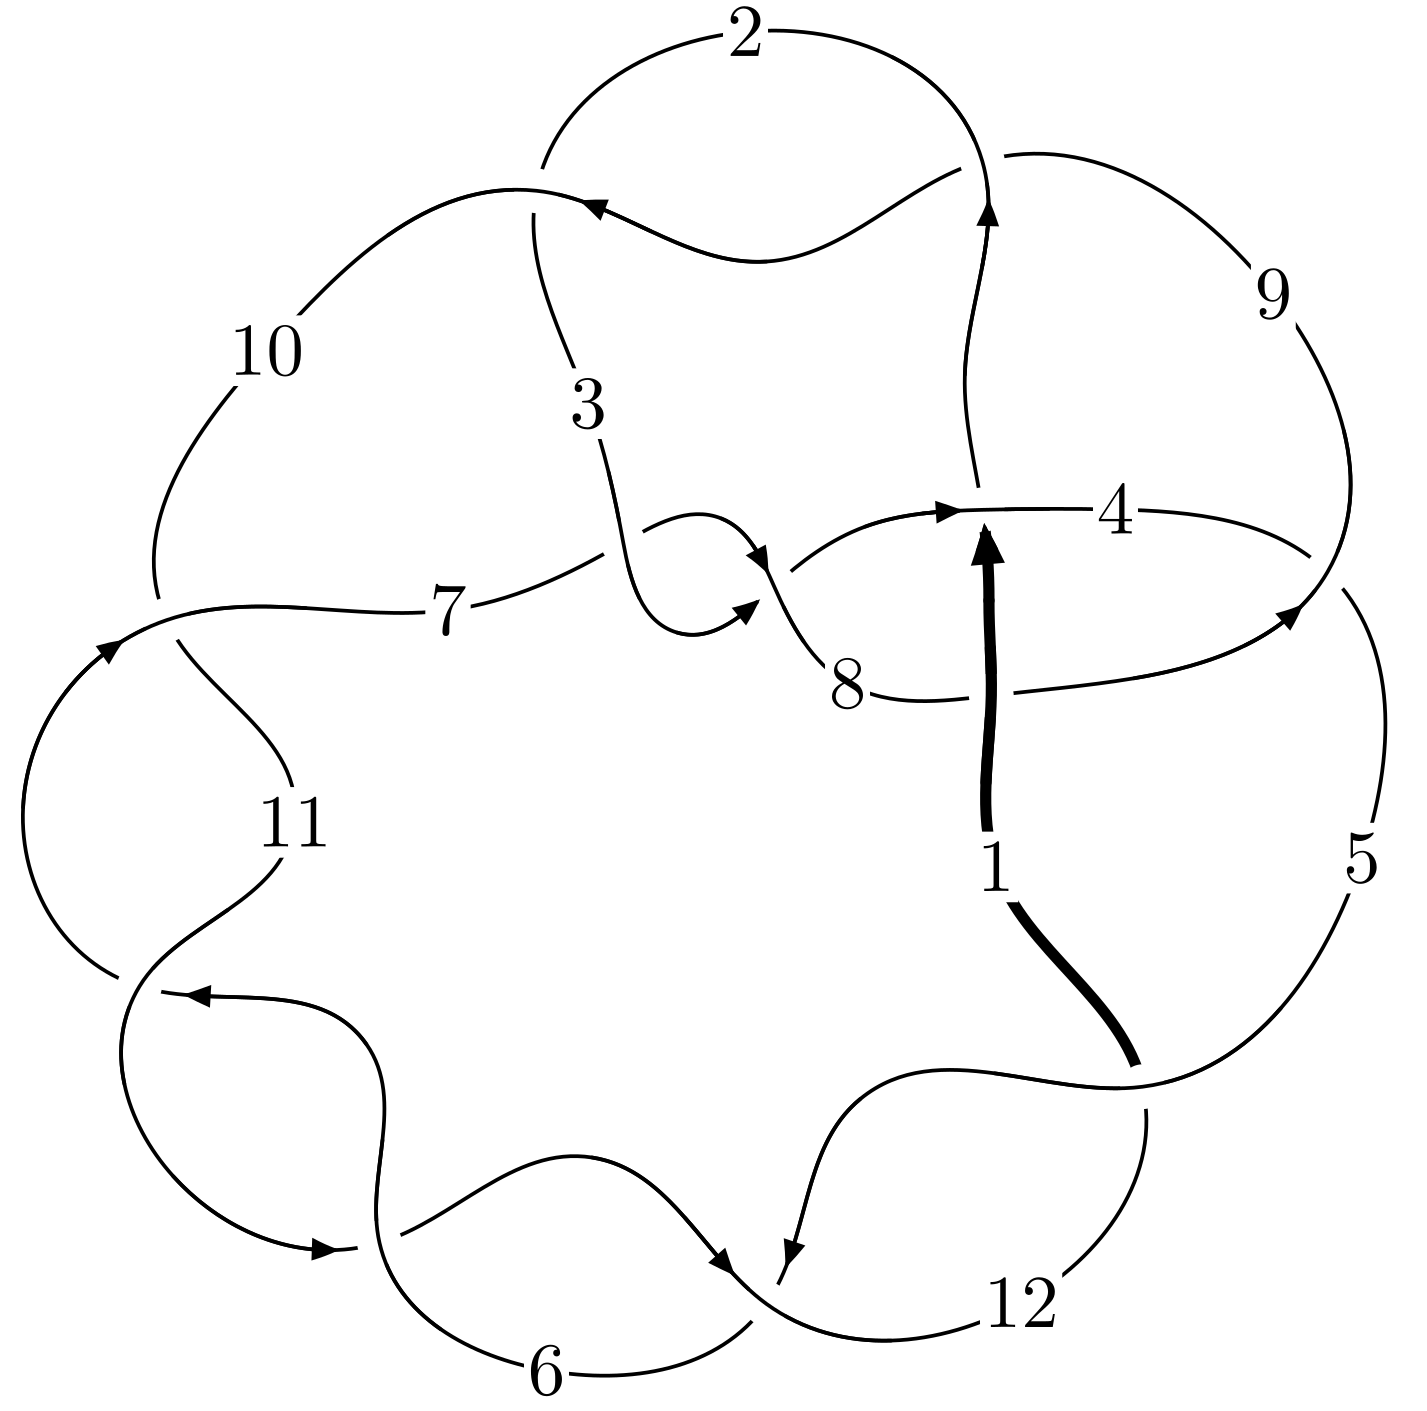
\includegraphics[width=112pt]{../../../GIT/diagram.site/Diagrams/png/1980_12a_1179.png}\\
\ \ \ A knot diagram\footnotemark}&
\allowdisplaybreaks
\textbf{Linearized knot diagam} \\
\cline{2-2}
 &
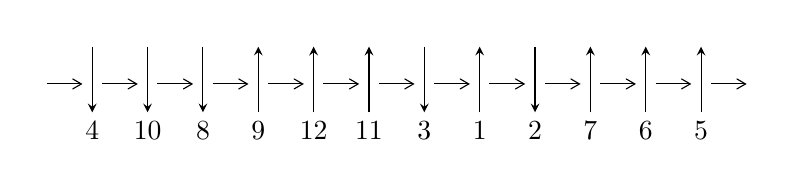
\begin{tikzpicture}[x=20pt, y=17pt]
	% nodes
	\node (C0) at (0, 0) {};
	\node (C1) at (1, 0) {};
	\node (C1U) at (1, +1) {};
	\node (C1D) at (1, -1) {4};

	\node (C2) at (2, 0) {};
	\node (C2U) at (2, +1) {};
	\node (C2D) at (2, -1) {10};

	\node (C3) at (3, 0) {};
	\node (C3U) at (3, +1) {};
	\node (C3D) at (3, -1) {8};

	\node (C4) at (4, 0) {};
	\node (C4U) at (4, +1) {};
	\node (C4D) at (4, -1) {9};

	\node (C5) at (5, 0) {};
	\node (C5U) at (5, +1) {};
	\node (C5D) at (5, -1) {12};

	\node (C6) at (6, 0) {};
	\node (C6U) at (6, +1) {};
	\node (C6D) at (6, -1) {11};

	\node (C7) at (7, 0) {};
	\node (C7U) at (7, +1) {};
	\node (C7D) at (7, -1) {3};

	\node (C8) at (8, 0) {};
	\node (C8U) at (8, +1) {};
	\node (C8D) at (8, -1) {1};

	\node (C9) at (9, 0) {};
	\node (C9U) at (9, +1) {};
	\node (C9D) at (9, -1) {2};

	\node (C10) at (10, 0) {};
	\node (C10U) at (10, +1) {};
	\node (C10D) at (10, -1) {7};

	\node (C11) at (11, 0) {};
	\node (C11U) at (11, +1) {};
	\node (C11D) at (11, -1) {6};

	\node (C12) at (12, 0) {};
	\node (C12U) at (12, +1) {};
	\node (C12D) at (12, -1) {5};
	\node (C13) at (13, 0) {};

	% arrows
	\draw[->,>={angle 60}]
	(C0) edge (C1) (C1) edge (C2) (C2) edge (C3) (C3) edge (C4) (C4) edge (C5) (C5) edge (C6) (C6) edge (C7) (C7) edge (C8) (C8) edge (C9) (C9) edge (C10) (C10) edge (C11) (C11) edge (C12) (C12) edge (C13) ;	\draw[->,>=stealth]
	(C1U) edge (C1D) (C2U) edge (C2D) (C3U) edge (C3D) (C4D) edge (C4U) (C5D) edge (C5U) (C6D) edge (C6U) (C7U) edge (C7D) (C8D) edge (C8U) (C9U) edge (C9D) (C10D) edge (C10U) (C11D) edge (C11U) (C12D) edge (C12U) ;
	\end{tikzpicture} \\
\hhline{~~} \\& 
\textbf{Solving Sequence} \\ \cline{2-2} 
 &
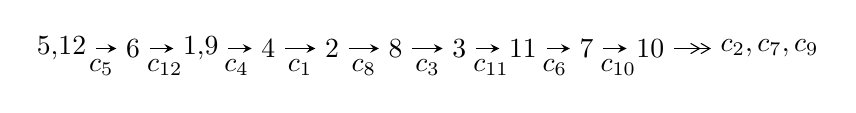
\begin{tikzpicture}[x=23pt, y=7pt]
	% node
	\node (A0) at (-1/8, 0) {5,12};
	\node (A1) at (1, 0) {6};
	\node (A2) at (33/16, 0) {1,9};
	\node (A3) at (25/8, 0) {4};
	\node (A4) at (33/8, 0) {2};
	\node (A5) at (41/8, 0) {8};
	\node (A6) at (49/8, 0) {3};
	\node (A7) at (57/8, 0) {11};
	\node (A8) at (65/8, 0) {7};
	\node (A9) at (73/8, 0) {10};
	\node (C1) at (1/2, -1) {$c_{5}$};
	\node (C2) at (3/2, -1) {$c_{12}$};
	\node (C3) at (21/8, -1) {$c_{4}$};
	\node (C4) at (29/8, -1) {$c_{1}$};
	\node (C5) at (37/8, -1) {$c_{8}$};
	\node (C6) at (45/8, -1) {$c_{3}$};
	\node (C7) at (53/8, -1) {$c_{11}$};
	\node (C8) at (61/8, -1) {$c_{6}$};
	\node (C9) at (69/8, -1) {$c_{10}$};
	\node (A10) at (11, 0) {$c_{2},c_{7},c_{9}$};

	% edge
	\draw[->,>=stealth]	
	(A0) edge (A1) (A1) edge (A2) (A2) edge (A3) (A3) edge (A4) (A4) edge (A5) (A5) edge (A6) (A6) edge (A7) (A7) edge (A8) (A8) edge (A9) ;
	\draw[->>,>={angle 60}]	
	(A9) edge (A10);
\end{tikzpicture} \\ 

\end{tabular} \\

\footnotetext{
The image of knot diagram is generated by the software ``\textbf{Draw programme}" developed by Andrew Bartholomew(\url{http://www.layer8.co.uk/maths/draw/index.htm\#Running-draw}), where we modified some parts for our purpose(\url{https://github.com/CATsTAILs/LinksPainter}).
}\phantom \\ \newline 
\centering \textbf{Ideals for irreducible components\footnotemark of $X_{\text{par}}$} 
 
\begin{align*}
I^u_{1}&=\langle 
-3 u^{21}-20 u^{20}+\cdots+2 b-36,\;3 u^{21}+17 u^{20}+\cdots+4 a-10,\;u^{22}+7 u^{21}+\cdots+88 u+8\rangle \\
I^u_{2}&=\langle 
-1208412097 a^5 u^5+1863706926 u^5 a^4+\cdots+88241195076 a-13422878124,\\
\phantom{I^u_{2}}&\phantom{= \langle  }6 a^5 u^5+4 u^5 a^4+\cdots-38 a-32,\;u^6- u^5+5 u^4-4 u^3+6 u^2-3 u+1\rangle \\
I^u_{3}&=\langle 
- u^{12}-9 u^{10}-30 u^8-45 u^6-29 u^4+u^3-6 u^2+b+2 u,\\
\phantom{I^u_{3}}&\phantom{= \langle  }- u^{12}- u^{11}-9 u^{10}-9 u^9-30 u^8-30 u^7-45 u^6-45 u^5-29 u^4-28 u^3-5 u^2+a-4 u+2,\\
\phantom{I^u_{3}}&\phantom{= \langle  }u^{13}+10 u^{11}+38 u^9+68 u^7+57 u^5- u^4+18 u^3-3 u^2-1\rangle \\
\\
\end{align*}
\raggedright * 3 irreducible components of $\dim_{\mathbb{C}}=0$, with total 71 representations.\\
\footnotetext{All coefficients of polynomials are rational numbers. But the coefficients are sometimes approximated in decimal forms when there is not enough margin.}
\newpage
\renewcommand{\arraystretch}{1}
\centering \section*{I. $I^u_{1}= \langle -3 u^{21}-20 u^{20}+\cdots+2 b-36,\;3 u^{21}+17 u^{20}+\cdots+4 a-10,\;u^{22}+7 u^{21}+\cdots+88 u+8 \rangle$}
\flushleft \textbf{(i) Arc colorings}\\
\begin{tabular}{m{7pt} m{180pt} m{7pt} m{180pt} }
\flushright $a_{5}=$&$\begin{pmatrix}1\\0\end{pmatrix}$ \\
\flushright $a_{12}=$&$\begin{pmatrix}0\\u\end{pmatrix}$ \\
\flushright $a_{6}=$&$\begin{pmatrix}1\\- u^2\end{pmatrix}$ \\
\flushright $a_{1}=$&$\begin{pmatrix}u\\u\end{pmatrix}$ \\
\flushright $a_{9}=$&$\begin{pmatrix}-\frac{3}{4} u^{21}-\frac{17}{4} u^{20}+\cdots+8 u+\frac{5}{2}\\\frac{3}{2} u^{21}+10 u^{20}+\cdots+\frac{365}{2} u+18\end{pmatrix}$ \\
\flushright $a_{4}=$&$\begin{pmatrix}\frac{1}{2} u^{21}+\frac{15}{4} u^{20}+\cdots+\frac{461}{4} u+13\\-\frac{1}{4} u^{21}-\frac{5}{4} u^{20}+\cdots-48 u-6\end{pmatrix}$ \\
\flushright $a_{2}=$&$\begin{pmatrix}\frac{3}{8} u^{21}+\frac{19}{8} u^{20}+\cdots+\frac{115}{2} u+\frac{13}{2}\\\frac{1}{4} u^{21}+\frac{7}{4} u^{20}+\cdots+\frac{23}{2} u+1\end{pmatrix}$ \\
\flushright $a_{8}=$&$\begin{pmatrix}-\frac{5}{4} u^{21}-\frac{31}{4} u^{20}+\cdots-106 u-\frac{19}{2}\\u^{21}+\frac{13}{2} u^{20}+\cdots+\frac{137}{2} u+6\end{pmatrix}$ \\
\flushright $a_{3}=$&$\begin{pmatrix}-\frac{3}{8} u^{21}-\frac{19}{8} u^{20}+\cdots-\frac{55}{2} u-\frac{5}{2}\\-\frac{1}{4} u^{21}-\frac{7}{4} u^{20}+\cdots-\frac{53}{2} u-3\end{pmatrix}$ \\
\flushright $a_{11}=$&$\begin{pmatrix}- u\\u^3+u\end{pmatrix}$ \\
\flushright $a_{7}=$&$\begin{pmatrix}u^2+1\\- u^4-2 u^2\end{pmatrix}$ \\
\flushright $a_{10}=$&$\begin{pmatrix}- u^3-2 u\\u^5+3 u^3+u\end{pmatrix}$\\&\end{tabular}
\flushleft \textbf{(ii) Obstruction class $= -1$}\\~\\
\flushleft \textbf{(iii) Cusp Shapes $= u^{20}+6 u^{19}+32 u^{18}+116 u^{17}+363 u^{16}+934 u^{15}+2100 u^{14}+4092 u^{13}+7035 u^{12}+10658 u^{11}+14285 u^{10}+16890 u^9+17584 u^8+15990 u^7+12628 u^6+8526 u^5+4861 u^4+2276 u^3+846 u^2+236 u+42$}\\~\\
\newpage\renewcommand{\arraystretch}{1}
\flushleft \textbf{(iv) u-Polynomials at the component}\newline \\
\begin{tabular}{m{50pt}|m{274pt}}
Crossings & \hspace{64pt}u-Polynomials at each crossing \\
\hline $$\begin{aligned}c_{1}\end{aligned}$$&$\begin{aligned}
&u^{22}-19 u^{21}+\cdots-800 u+64
\end{aligned}$\\
\hline $$\begin{aligned}c_{2},c_{3},c_{7}\\c_{9}\end{aligned}$$&$\begin{aligned}
&u^{22}- u^{21}+\cdots+6 u^2+1
\end{aligned}$\\
\hline $$\begin{aligned}c_{4},c_{8}\end{aligned}$$&$\begin{aligned}
&u^{22}+6 u^{20}+\cdots- u+1
\end{aligned}$\\
\hline $$\begin{aligned}c_{5},c_{6},c_{10}\\c_{11},c_{12}\end{aligned}$$&$\begin{aligned}
&u^{22}-7 u^{21}+\cdots-88 u+8
\end{aligned}$\\
\hline
\end{tabular}\\~\\
\newpage\renewcommand{\arraystretch}{1}
\flushleft \textbf{(v) Riley Polynomials at the component}\newline \\
\begin{tabular}{m{50pt}|m{274pt}}
Crossings & \hspace{64pt}Riley Polynomials at each crossing \\
\hline $$\begin{aligned}c_{1}\end{aligned}$$&$\begin{aligned}
&y^{22}- y^{21}+\cdots-1024 y+4096
\end{aligned}$\\
\hline $$\begin{aligned}c_{2},c_{3},c_{7}\\c_{9}\end{aligned}$$&$\begin{aligned}
&y^{22}-25 y^{21}+\cdots+12 y+1
\end{aligned}$\\
\hline $$\begin{aligned}c_{4},c_{8}\end{aligned}$$&$\begin{aligned}
&y^{22}+12 y^{21}+\cdots-7 y+1
\end{aligned}$\\
\hline $$\begin{aligned}c_{5},c_{6},c_{10}\\c_{11},c_{12}\end{aligned}$$&$\begin{aligned}
&y^{22}+29 y^{21}+\cdots+32 y+64
\end{aligned}$\\
\hline
\end{tabular}\\~\\
\newpage\flushleft \textbf{(vi) Complex Volumes and Cusp Shapes}
$$\begin{array}{c|c|c}  
\text{Solutions to }I^u_{1}& \I (\text{vol} + \sqrt{-1}CS) & \text{Cusp shape}\\
 \hline 
\begin{aligned}
u &= -0.214951 + 0.955332 I \\
a &= -0.39803 - 1.38319 I \\
b &= \phantom{-}0.670593 - 0.921685 I\end{aligned}
 & -2.60701 - 2.88422 I & -0.19154 + 3.17334 I \\ \hline\begin{aligned}
u &= -0.214951 - 0.955332 I \\
a &= -0.39803 + 1.38319 I \\
b &= \phantom{-}0.670593 + 0.921685 I\end{aligned}
 & -2.60701 + 2.88422 I & -0.19154 - 3.17334 I \\ \hline\begin{aligned}
u &= -0.813603 + 0.334821 I \\
a &= -0.391314 + 0.249585 I \\
b &= -0.463678 - 0.959425 I\end{aligned}
 & -6.77494 + 2.66525 I & -5.93834 - 2.44908 I \\ \hline\begin{aligned}
u &= -0.813603 - 0.334821 I \\
a &= -0.391314 - 0.249585 I \\
b &= -0.463678 + 0.959425 I\end{aligned}
 & -6.77494 - 2.66525 I & -5.93834 + 2.44908 I \\ \hline\begin{aligned}
u &= -0.722432 + 0.499538 I \\
a &= -0.667442 - 0.524436 I \\
b &= \phantom{-}0.702002 - 1.099620 I\end{aligned}
 & -7.31468 - 7.59742 I & -4.88198 + 6.88559 I \\ \hline\begin{aligned}
u &= -0.722432 - 0.499538 I \\
a &= -0.667442 + 0.524436 I \\
b &= \phantom{-}0.702002 + 1.099620 I\end{aligned}
 & -7.31468 + 7.59742 I & -4.88198 - 6.88559 I \\ \hline\begin{aligned}
u &= -0.386869 + 1.238110 I \\
a &= \phantom{-}0.29217 + 1.62873 I \\
b &= -0.85810 + 1.29508 I\end{aligned}
 & -12.8000 - 11.4299 I & -6.89165 + 6.89710 I \\ \hline\begin{aligned}
u &= -0.386869 - 1.238110 I \\
a &= \phantom{-}0.29217 - 1.62873 I \\
b &= -0.85810 - 1.29508 I\end{aligned}
 & -12.8000 + 11.4299 I & -6.89165 - 6.89710 I \\ \hline\begin{aligned}
u &= -0.518713 + 1.209380 I \\
a &= \phantom{-}0.749140 + 0.553517 I \\
b &= \phantom{-}0.141219 + 0.931028 I\end{aligned}
 & -11.52230 - 1.93620 I & -10.29123 + 1.11937 I \\ \hline\begin{aligned}
u &= -0.518713 - 1.209380 I \\
a &= \phantom{-}0.749140 - 0.553517 I \\
b &= \phantom{-}0.141219 - 0.931028 I\end{aligned}
 & -11.52230 + 1.93620 I & -10.29123 - 1.11937 I\\
 \hline 
 \end{array}$$\newpage$$\begin{array}{c|c|c}  
\text{Solutions to }I^u_{1}& \I (\text{vol} + \sqrt{-1}CS) & \text{Cusp shape}\\
 \hline 
\begin{aligned}
u &= -0.188904 + 0.563822 I \\
a &= \phantom{-}0.341201 - 0.743824 I \\
b &= \phantom{-}0.487380 + 0.071622 I\end{aligned}
 & -0.321406 - 1.315600 I & \phantom{-}0.42346 + 6.52764 I \\ \hline\begin{aligned}
u &= -0.188904 - 0.563822 I \\
a &= \phantom{-}0.341201 + 0.743824 I \\
b &= \phantom{-}0.487380 - 0.071622 I\end{aligned}
 & -0.321406 + 1.315600 I & \phantom{-}0.42346 - 6.52764 I \\ \hline\begin{aligned}
u &= \phantom{-}0.03206 + 1.53855 I \\
a &= -0.320508 + 0.481993 I \\
b &= -0.440190 + 0.193391 I\end{aligned}
 & -7.43727 - 1.58134 I & \phantom{-}0.15073 + 4.91907 I \\ \hline\begin{aligned}
u &= \phantom{-}0.03206 - 1.53855 I \\
a &= -0.320508 - 0.481993 I \\
b &= -0.440190 - 0.193391 I\end{aligned}
 & -7.43727 + 1.58134 I & \phantom{-}0.15073 - 4.91907 I \\ \hline\begin{aligned}
u &= -0.398382 + 0.163640 I \\
a &= \phantom{-}1.041370 - 0.104922 I \\
b &= -0.526173 + 0.495850 I\end{aligned}
 & \phantom{-}0.836027 - 0.793326 I & \phantom{-}6.74273 + 3.41727 I \\ \hline\begin{aligned}
u &= -0.398382 - 0.163640 I \\
a &= \phantom{-}1.041370 + 0.104922 I \\
b &= -0.526173 - 0.495850 I\end{aligned}
 & \phantom{-}0.836027 + 0.793326 I & \phantom{-}6.74273 - 3.41727 I \\ \hline\begin{aligned}
u &= -0.05207 + 1.70520 I \\
a &= -0.13197 + 1.64255 I \\
b &= -0.83496 + 1.17436 I\end{aligned}
 & -12.05740 - 3.92251 I & \phantom{-}0.689774 + 0.408842 I \\ \hline\begin{aligned}
u &= -0.05207 - 1.70520 I \\
a &= -0.13197 - 1.64255 I \\
b &= -0.83496 - 1.17436 I\end{aligned}
 & -12.05740 + 3.92251 I & \phantom{-}0.689774 - 0.408842 I \\ \hline\begin{aligned}
u &= -0.10228 + 1.79386 I \\
a &= \phantom{-}0.12610 - 1.92859 I \\
b &= \phantom{-}0.95775 - 1.44210 I\end{aligned}
 & \phantom{-}15.7405 - 13.6253 I & -7.26879 + 5.92995 I \\ \hline\begin{aligned}
u &= -0.10228 - 1.79386 I \\
a &= \phantom{-}0.12610 + 1.92859 I \\
b &= \phantom{-}0.95775 + 1.44210 I\end{aligned}
 & \phantom{-}15.7405 + 13.6253 I & -7.26879 - 5.92995 I\\
 \hline 
 \end{array}$$\newpage$$\begin{array}{c|c|c}  
\text{Solutions to }I^u_{1}& \I (\text{vol} + \sqrt{-1}CS) & \text{Cusp shape}\\
 \hline 
\begin{aligned}
u &= -0.13386 + 1.80777 I \\
a &= -0.390730 - 1.046170 I \\
b &= \phantom{-}0.164157 - 0.996452 I\end{aligned}
 & \phantom{-}17.1171 - 4.8585 I & -9.54317 + 2.73303 I \\ \hline\begin{aligned}
u &= -0.13386 - 1.80777 I \\
a &= -0.390730 + 1.046170 I \\
b &= \phantom{-}0.164157 + 0.996452 I\end{aligned}
 & \phantom{-}17.1171 + 4.8585 I & -9.54317 - 2.73303 I\\
 \hline 
 \end{array}$$\newpage\newpage\renewcommand{\arraystretch}{1}
\centering \section*{II. $I^u_{2}= \langle -1.21\times10^{9} a^{5} u^{5}+1.86\times10^{9} a^{4} u^{5}+\cdots+8.82\times10^{10} a-1.34\times10^{10},\;6 a^5 u^5+4 u^5 a^4+\cdots-38 a-32,\;u^6- u^5+5 u^4-4 u^3+6 u^2-3 u+1 \rangle$}
\flushleft \textbf{(i) Arc colorings}\\
\begin{tabular}{m{7pt} m{180pt} m{7pt} m{180pt} }
\flushright $a_{5}=$&$\begin{pmatrix}1\\0\end{pmatrix}$ \\
\flushright $a_{12}=$&$\begin{pmatrix}0\\u\end{pmatrix}$ \\
\flushright $a_{6}=$&$\begin{pmatrix}1\\- u^2\end{pmatrix}$ \\
\flushright $a_{1}=$&$\begin{pmatrix}u\\u\end{pmatrix}$ \\
\flushright $a_{9}=$&$\begin{pmatrix}a\\0.372194 a^{5} u^{5}-0.574026 a^{4} u^{5}+\cdots-27.1785 a+4.13428\end{pmatrix}$ \\
\flushright $a_{4}=$&$\begin{pmatrix}-0.145773 a^{5} u^{5}+2.18213 a^{4} u^{5}+\cdots+17.8628 a-21.1907\\0.312265 a^{5} u^{5}-1.60138 a^{4} u^{5}+\cdots-34.5790 a+1.77561\end{pmatrix}$ \\
\flushright $a_{2}=$&$\begin{pmatrix}-0.206418 a^{5} u^{5}-2.57431 a^{4} u^{5}+\cdots-10.7722 a+16.8693\\0.110381 a^{5} u^{5}-0.378957 a^{4} u^{5}+\cdots-20.5376 a-6.45733\end{pmatrix}$ \\
\flushright $a_{8}=$&$\begin{pmatrix}0.132970 a^{5} u^{5}+1.05447 a^{4} u^{5}+\cdots+1.43345 a-5.94094\\0.505164 a^{5} u^{5}+0.480448 a^{4} u^{5}+\cdots-26.7451 a-1.80666\end{pmatrix}$ \\
\flushright $a_{3}=$&$\begin{pmatrix}-0.0660601 a^{5} u^{5}+1.04617 a^{4} u^{5}+\cdots+12.8011 a-4.58028\\-0.295252 a^{5} u^{5}+0.333319 a^{4} u^{5}+\cdots+13.4971 a+1.63976\end{pmatrix}$ \\
\flushright $a_{11}=$&$\begin{pmatrix}- u\\u^3+u\end{pmatrix}$ \\
\flushright $a_{7}=$&$\begin{pmatrix}u^2+1\\- u^4-2 u^2\end{pmatrix}$ \\
\flushright $a_{10}=$&$\begin{pmatrix}- u^3-2 u\\u^5+3 u^3+u\end{pmatrix}$\\&\end{tabular}
\flushleft \textbf{(ii) Obstruction class $= -1$}\\~\\
\flushleft \textbf{(iii) Cusp Shapes $= -\frac{10836912}{649345301} a^5 u^5+\frac{6217485248}{649345301} u^5 a^4+\cdots+\frac{27178566568}{649345301} a-\frac{51617037366}{649345301}$}\\~\\
\newpage\renewcommand{\arraystretch}{1}
\flushleft \textbf{(iv) u-Polynomials at the component}\newline \\
\begin{tabular}{m{50pt}|m{274pt}}
Crossings & \hspace{64pt}u-Polynomials at each crossing \\
\hline $$\begin{aligned}c_{1}\end{aligned}$$&$\begin{aligned}
&(u^3+u^2-1)^{12}
\end{aligned}$\\
\hline $$\begin{aligned}c_{2},c_{3},c_{7}\\c_{9}\end{aligned}$$&$\begin{aligned}
&u^{36}+u^{35}+\cdots-334 u+77
\end{aligned}$\\
\hline $$\begin{aligned}c_{4},c_{8}\end{aligned}$$&$\begin{aligned}
&u^{36}+3 u^{35}+\cdots+244 u+271
\end{aligned}$\\
\hline $$\begin{aligned}c_{5},c_{6},c_{10}\\c_{11},c_{12}\end{aligned}$$&$\begin{aligned}
&(u^6+u^5+5 u^4+4 u^3+6 u^2+3 u+1)^6
\end{aligned}$\\
\hline
\end{tabular}\\~\\
\newpage\renewcommand{\arraystretch}{1}
\flushleft \textbf{(v) Riley Polynomials at the component}\newline \\
\begin{tabular}{m{50pt}|m{274pt}}
Crossings & \hspace{64pt}Riley Polynomials at each crossing \\
\hline $$\begin{aligned}c_{1}\end{aligned}$$&$\begin{aligned}
&(y^3- y^2+2 y-1)^{12}
\end{aligned}$\\
\hline $$\begin{aligned}c_{2},c_{3},c_{7}\\c_{9}\end{aligned}$$&$\begin{aligned}
&y^{36}-33 y^{35}+\cdots+209380 y+5929
\end{aligned}$\\
\hline $$\begin{aligned}c_{4},c_{8}\end{aligned}$$&$\begin{aligned}
&y^{36}+11 y^{35}+\cdots+1542616 y+73441
\end{aligned}$\\
\hline $$\begin{aligned}c_{5},c_{6},c_{10}\\c_{11},c_{12}\end{aligned}$$&$\begin{aligned}
&(y^6+9 y^5+29 y^4+40 y^3+22 y^2+3 y+1)^6
\end{aligned}$\\
\hline
\end{tabular}\\~\\
\newpage\flushleft \textbf{(vi) Complex Volumes and Cusp Shapes}
$$\begin{array}{c|c|c}  
\text{Solutions to }I^u_{2}& \I (\text{vol} + \sqrt{-1}CS) & \text{Cusp shape}\\
 \hline 
\begin{aligned}
u &= \phantom{-}0.142924 + 1.159520 I \\
a &= \phantom{-}0.020396 - 0.755302 I \\
b &= -0.624535 - 0.897322 I\end{aligned}
 & -6.55350 - 0.17216 I & -6.07139 - 0.41864 I \\ \hline\begin{aligned}
u &= \phantom{-}0.142924 + 1.159520 I \\
a &= -0.90019 + 1.20470 I \\
b &= -0.072498 + 0.768105 I\end{aligned}
 & -6.55350 - 0.17216 I & -6.07139 - 0.41864 I \\ \hline\begin{aligned}
u &= \phantom{-}0.142924 + 1.159520 I \\
a &= -1.09844 + 1.21563 I \\
b &= -1.70363 + 1.17475 I\end{aligned}
 & -10.69110 + 2.65597 I & -12.60066 - 3.39809 I \\ \hline\begin{aligned}
u &= \phantom{-}0.142924 + 1.159520 I \\
a &= \phantom{-}0.71837 - 1.49821 I \\
b &= -0.702328 - 0.883472 I\end{aligned}
 & -6.55350 + 5.48409 I & -6.07139 - 6.37753 I \\ \hline\begin{aligned}
u &= \phantom{-}0.142924 + 1.159520 I \\
a &= \phantom{-}0.09177 + 2.06359 I \\
b &= \phantom{-}0.91585 + 1.55946 I\end{aligned}
 & -6.55350 + 5.48409 I & -6.07139 - 6.37753 I \\ \hline\begin{aligned}
u &= \phantom{-}0.142924 + 1.159520 I \\
a &= \phantom{-}0.85867 + 2.27785 I \\
b &= \phantom{-}0.039086 + 0.707567 I\end{aligned}
 & -10.69110 + 2.65597 I & -12.60066 - 3.39809 I \\ \hline\begin{aligned}
u &= \phantom{-}0.142924 - 1.159520 I \\
a &= \phantom{-}0.020396 + 0.755302 I \\
b &= -0.624535 + 0.897322 I\end{aligned}
 & -6.55350 + 0.17216 I & -6.07139 + 0.41864 I \\ \hline\begin{aligned}
u &= \phantom{-}0.142924 - 1.159520 I \\
a &= -0.90019 - 1.20470 I \\
b &= -0.072498 - 0.768105 I\end{aligned}
 & -6.55350 + 0.17216 I & -6.07139 + 0.41864 I \\ \hline\begin{aligned}
u &= \phantom{-}0.142924 - 1.159520 I \\
a &= -1.09844 - 1.21563 I \\
b &= -1.70363 - 1.17475 I\end{aligned}
 & -10.69110 - 2.65597 I & -12.60066 + 3.39809 I \\ \hline\begin{aligned}
u &= \phantom{-}0.142924 - 1.159520 I \\
a &= \phantom{-}0.71837 + 1.49821 I \\
b &= -0.702328 + 0.883472 I\end{aligned}
 & -6.55350 - 5.48409 I & -6.07139 + 6.37753 I\\
 \hline 
 \end{array}$$\newpage$$\begin{array}{c|c|c}  
\text{Solutions to }I^u_{2}& \I (\text{vol} + \sqrt{-1}CS) & \text{Cusp shape}\\
 \hline 
\begin{aligned}
u &= \phantom{-}0.142924 - 1.159520 I \\
a &= \phantom{-}0.09177 - 2.06359 I \\
b &= \phantom{-}0.91585 - 1.55946 I\end{aligned}
 & -6.55350 - 5.48409 I & -6.07139 + 6.37753 I \\ \hline\begin{aligned}
u &= \phantom{-}0.142924 - 1.159520 I \\
a &= \phantom{-}0.85867 - 2.27785 I \\
b &= \phantom{-}0.039086 - 0.707567 I\end{aligned}
 & -10.69110 - 2.65597 I & -12.60066 + 3.39809 I \\ \hline\begin{aligned}
u &= \phantom{-}0.321608 + 0.359079 I \\
a &= -0.541913 - 0.991237 I \\
b &= \phantom{-}1.134260 - 0.815115 I\end{aligned}
 & -5.79017 + 1.10871 I & -7.48336 - 6.18117 I \\ \hline\begin{aligned}
u &= \phantom{-}0.321608 + 0.359079 I \\
a &= -0.573836 - 1.111540 I \\
b &= -0.036630 + 0.730558 I\end{aligned}
 & -1.65258 - 1.71942 I & -0.95409 - 3.20172 I \\ \hline\begin{aligned}
u &= \phantom{-}0.321608 + 0.359079 I \\
a &= \phantom{-}1.120820 - 0.796180 I \\
b &= -0.727819 - 1.151300 I\end{aligned}
 & -1.65258 + 3.93683 I & -0.95409 - 9.16062 I \\ \hline\begin{aligned}
u &= \phantom{-}0.321608 + 0.359079 I \\
a &= \phantom{-}1.56692 + 0.28239 I \\
b &= \phantom{-}0.488689 - 0.785333 I\end{aligned}
 & -1.65258 - 1.71942 I & -0.95409 - 3.20172 I \\ \hline\begin{aligned}
u &= \phantom{-}0.321608 + 0.359079 I \\
a &= -2.31941 + 0.30926 I \\
b &= \phantom{-}0.467021 + 0.778019 I\end{aligned}
 & -1.65258 + 3.93683 I & -0.95409 - 9.16062 I \\ \hline\begin{aligned}
u &= \phantom{-}0.321608 + 0.359079 I \\
a &= -0.16556 - 3.53944 I \\
b &= -0.475830 - 0.658521 I\end{aligned}
 & -5.79017 + 1.10871 I & -7.48336 - 6.18117 I \\ \hline\begin{aligned}
u &= \phantom{-}0.321608 - 0.359079 I \\
a &= -0.541913 + 0.991237 I \\
b &= \phantom{-}1.134260 + 0.815115 I\end{aligned}
 & -5.79017 - 1.10871 I & -7.48336 + 6.18117 I \\ \hline\begin{aligned}
u &= \phantom{-}0.321608 - 0.359079 I \\
a &= -0.573836 + 1.111540 I \\
b &= -0.036630 - 0.730558 I\end{aligned}
 & -1.65258 + 1.71942 I & -0.95409 + 3.20172 I\\
 \hline 
 \end{array}$$\newpage$$\begin{array}{c|c|c}  
\text{Solutions to }I^u_{2}& \I (\text{vol} + \sqrt{-1}CS) & \text{Cusp shape}\\
 \hline 
\begin{aligned}
u &= \phantom{-}0.321608 - 0.359079 I \\
a &= \phantom{-}1.120820 + 0.796180 I \\
b &= -0.727819 + 1.151300 I\end{aligned}
 & -1.65258 - 3.93683 I & -0.95409 + 9.16062 I \\ \hline\begin{aligned}
u &= \phantom{-}0.321608 - 0.359079 I \\
a &= \phantom{-}1.56692 - 0.28239 I \\
b &= \phantom{-}0.488689 + 0.785333 I\end{aligned}
 & -1.65258 + 1.71942 I & -0.95409 + 3.20172 I \\ \hline\begin{aligned}
u &= \phantom{-}0.321608 - 0.359079 I \\
a &= -2.31941 - 0.30926 I \\
b &= \phantom{-}0.467021 - 0.778019 I\end{aligned}
 & -1.65258 - 3.93683 I & -0.95409 + 9.16062 I \\ \hline\begin{aligned}
u &= \phantom{-}0.321608 - 0.359079 I \\
a &= -0.16556 + 3.53944 I \\
b &= -0.475830 + 0.658521 I\end{aligned}
 & -5.79017 - 1.10871 I & -7.48336 + 6.18117 I \\ \hline\begin{aligned}
u &= \phantom{-}0.03547 + 1.77530 I \\
a &= \phantom{-}0.483101 + 1.162360 I \\
b &= \phantom{-}0.98695 + 1.09529 I\end{aligned}
 & -17.2652 + 0.5991 I & -6.44525 + 0.72721 I \\ \hline\begin{aligned}
u &= \phantom{-}0.03547 + 1.77530 I \\
a &= \phantom{-}0.49089 - 1.43550 I \\
b &= -0.136931 - 0.892105 I\end{aligned}
 & -17.2652 + 0.5991 I & -6.44525 + 0.72721 I \\ \hline\begin{aligned}
u &= \phantom{-}0.03547 + 1.77530 I \\
a &= -0.19050 + 1.53203 I \\
b &= \phantom{-}0.836637 + 0.957299 I\end{aligned}
 & -17.2652 + 6.2553 I & -6.44525 - 5.23168 I \\ \hline\begin{aligned}
u &= \phantom{-}0.03547 + 1.77530 I \\
a &= -0.63078 - 1.91690 I \\
b &= \phantom{-}0.159090 - 0.769263 I\end{aligned}
 & \phantom{-}18.0757 + 3.4272 I & -12.97451 - 2.25224 I \\ \hline\begin{aligned}
u &= \phantom{-}0.03547 + 1.77530 I \\
a &= \phantom{-}1.57803 - 1.54119 I \\
b &= \phantom{-}2.00938 - 1.44296 I\end{aligned}
 & \phantom{-}18.0757 + 3.4272 I & -12.97451 - 2.25224 I \\ \hline\begin{aligned}
u &= \phantom{-}0.03547 + 1.77530 I \\
a &= -0.50833 - 2.26340 I \\
b &= -1.05676 - 1.80309 I\end{aligned}
 & -17.2652 + 6.2553 I & -6.44525 - 5.23168 I\\
 \hline 
 \end{array}$$\newpage$$\begin{array}{c|c|c}  
\text{Solutions to }I^u_{2}& \I (\text{vol} + \sqrt{-1}CS) & \text{Cusp shape}\\
 \hline 
\begin{aligned}
u &= \phantom{-}0.03547 - 1.77530 I \\
a &= \phantom{-}0.483101 - 1.162360 I \\
b &= \phantom{-}0.98695 - 1.09529 I\end{aligned}
 & -17.2652 - 0.5991 I & -6.44525 - 0.72721 I \\ \hline\begin{aligned}
u &= \phantom{-}0.03547 - 1.77530 I \\
a &= \phantom{-}0.49089 + 1.43550 I \\
b &= -0.136931 + 0.892105 I\end{aligned}
 & -17.2652 - 0.5991 I & -6.44525 - 0.72721 I \\ \hline\begin{aligned}
u &= \phantom{-}0.03547 - 1.77530 I \\
a &= -0.19050 - 1.53203 I \\
b &= \phantom{-}0.836637 - 0.957299 I\end{aligned}
 & -17.2652 - 6.2553 I & -6.44525 + 5.23168 I \\ \hline\begin{aligned}
u &= \phantom{-}0.03547 - 1.77530 I \\
a &= -0.63078 + 1.91690 I \\
b &= \phantom{-}0.159090 + 0.769263 I\end{aligned}
 & \phantom{-}18.0757 - 3.4272 I & -12.97451 + 2.25224 I \\ \hline\begin{aligned}
u &= \phantom{-}0.03547 - 1.77530 I \\
a &= \phantom{-}1.57803 + 1.54119 I \\
b &= \phantom{-}2.00938 + 1.44296 I\end{aligned}
 & \phantom{-}18.0757 - 3.4272 I & -12.97451 + 2.25224 I \\ \hline\begin{aligned}
u &= \phantom{-}0.03547 - 1.77530 I \\
a &= -0.50833 + 2.26340 I \\
b &= -1.05676 + 1.80309 I\end{aligned}
 & -17.2652 - 6.2553 I & -6.44525 + 5.23168 I\\
 \hline 
 \end{array}$$\newpage\newpage\renewcommand{\arraystretch}{1}
\centering \section*{III. $I^u_{3}= \langle - u^{12}-9 u^{10}+\cdots+b+2 u,\;- u^{12}- u^{11}+\cdots+a+2,\;u^{13}+10 u^{11}+\cdots-3 u^2-1 \rangle$}
\flushleft \textbf{(i) Arc colorings}\\
\begin{tabular}{m{7pt} m{180pt} m{7pt} m{180pt} }
\flushright $a_{5}=$&$\begin{pmatrix}1\\0\end{pmatrix}$ \\
\flushright $a_{12}=$&$\begin{pmatrix}0\\u\end{pmatrix}$ \\
\flushright $a_{6}=$&$\begin{pmatrix}1\\- u^2\end{pmatrix}$ \\
\flushright $a_{1}=$&$\begin{pmatrix}u\\u\end{pmatrix}$ \\
\flushright $a_{9}=$&$\begin{pmatrix}u^{12}+u^{11}+\cdots+4 u-2\\u^{12}+9 u^{10}+30 u^8+45 u^6+29 u^4- u^3+6 u^2-2 u\end{pmatrix}$ \\
\flushright $a_{4}=$&$\begin{pmatrix}- u^{12}-10 u^{10}+\cdots+5 u+2\\u^9+7 u^7+16 u^5+13 u^3+2 u-1\end{pmatrix}$ \\
\flushright $a_{2}=$&$\begin{pmatrix}- u^{12}-10 u^{10}+\cdots-3 u+2\\u^9- u^8+7 u^7-6 u^6+16 u^5-11 u^4+13 u^3-6 u^2+3 u-1\end{pmatrix}$ \\
\flushright $a_{8}=$&$\begin{pmatrix}u^{12}+9 u^{10}+\cdots+4 u-1\\u^{12}- u^{11}+\cdots-2 u+1\end{pmatrix}$ \\
\flushright $a_{3}=$&$\begin{pmatrix}- u^{12}-10 u^{10}-38 u^8-67 u^6- u^5-52 u^4-3 u^3-11 u^2- u+2\\- u^8+u^7-6 u^6+5 u^5-11 u^4+7 u^3-6 u^2+2 u-1\end{pmatrix}$ \\
\flushright $a_{11}=$&$\begin{pmatrix}- u\\u^3+u\end{pmatrix}$ \\
\flushright $a_{7}=$&$\begin{pmatrix}u^2+1\\- u^4-2 u^2\end{pmatrix}$ \\
\flushright $a_{10}=$&$\begin{pmatrix}- u^3-2 u\\u^5+3 u^3+u\end{pmatrix}$\\&\end{tabular}
\flushleft \textbf{(ii) Obstruction class $= 1$}\\~\\
\flushleft \textbf{(iii) Cusp Shapes $= - u^{11}+u^{10}-11 u^9+11 u^8-44 u^7+40 u^6-77 u^5+57 u^4-55 u^3+28 u^2-10 u-4$}\\~\\
\newpage\renewcommand{\arraystretch}{1}
\flushleft \textbf{(iv) u-Polynomials at the component}\newline \\
\begin{tabular}{m{50pt}|m{274pt}}
Crossings & \hspace{64pt}u-Polynomials at each crossing \\
\hline $$\begin{aligned}c_{1}\end{aligned}$$&$\begin{aligned}
&u^{13}-4 u^{12}+8 u^{11}-8 u^{10}+u^9+7 u^8-5 u^7-3 u^6+3 u^5+4 u^4-4 u^3+1
\end{aligned}$\\
\hline $$\begin{aligned}c_{2},c_{7}\end{aligned}$$&$\begin{aligned}
&u^{13}+u^{12}+\cdots+u+1
\end{aligned}$\\
\hline $$\begin{aligned}c_{3},c_{9}\end{aligned}$$&$\begin{aligned}
&u^{13}- u^{12}+\cdots+u-1
\end{aligned}$\\
\hline $$\begin{aligned}c_{4},c_{8}\end{aligned}$$&$\begin{aligned}
&u^{13}+2 u^{11}- u^{10}+5 u^9- u^8+3 u^7+3 u^5+u^4+u^3-2 u^2-1
\end{aligned}$\\
\hline $$\begin{aligned}c_{5},c_{6}\end{aligned}$$&$\begin{aligned}
&u^{13}+10 u^{11}+38 u^9+68 u^7+57 u^5- u^4+18 u^3-3 u^2-1
\end{aligned}$\\
\hline $$\begin{aligned}c_{10},c_{11},c_{12}\end{aligned}$$&$\begin{aligned}
&u^{13}+10 u^{11}+38 u^9+68 u^7+57 u^5+u^4+18 u^3+3 u^2+1
\end{aligned}$\\
\hline
\end{tabular}\\~\\
\newpage\renewcommand{\arraystretch}{1}
\flushleft \textbf{(v) Riley Polynomials at the component}\newline \\
\begin{tabular}{m{50pt}|m{274pt}}
Crossings & \hspace{64pt}Riley Polynomials at each crossing \\
\hline $$\begin{aligned}c_{1}\end{aligned}$$&$\begin{aligned}
&y^{13}+2 y^{11}+\cdots-8 y^2-1
\end{aligned}$\\
\hline $$\begin{aligned}c_{2},c_{3},c_{7}\\c_{9}\end{aligned}$$&$\begin{aligned}
&y^{13}-13 y^{12}+\cdots+9 y-1
\end{aligned}$\\
\hline $$\begin{aligned}c_{4},c_{8}\end{aligned}$$&$\begin{aligned}
&y^{13}+4 y^{12}+\cdots-4 y-1
\end{aligned}$\\
\hline $$\begin{aligned}c_{5},c_{6},c_{10}\\c_{11},c_{12}\end{aligned}$$&$\begin{aligned}
&y^{13}+20 y^{12}+\cdots-6 y-1
\end{aligned}$\\
\hline
\end{tabular}\\~\\
\newpage\flushleft \textbf{(vi) Complex Volumes and Cusp Shapes}
$$\begin{array}{c|c|c}  
\text{Solutions to }I^u_{3}& \I (\text{vol} + \sqrt{-1}CS) & \text{Cusp shape}\\
 \hline 
\begin{aligned}
u &= \phantom{-}0.222851 + 1.128390 I \\
a &= -0.528316 + 1.119370 I \\
b &= -0.751183 + 0.409643 I\end{aligned}
 & -9.46673 + 2.12086 I & -5.40296 - 0.71019 I \\ \hline\begin{aligned}
u &= \phantom{-}0.222851 - 1.128390 I \\
a &= -0.528316 - 1.119370 I \\
b &= -0.751183 - 0.409643 I\end{aligned}
 & -9.46673 - 2.12086 I & -5.40296 + 0.71019 I \\ \hline\begin{aligned}
u &= -0.132288 + 0.825196 I \\
a &= -0.80812 - 1.63198 I \\
b &= \phantom{-}0.620126 - 1.109460 I\end{aligned}
 & -3.74892 - 3.58419 I & -7.53140 + 5.11211 I \\ \hline\begin{aligned}
u &= -0.132288 - 0.825196 I \\
a &= -0.80812 + 1.63198 I \\
b &= \phantom{-}0.620126 + 1.109460 I\end{aligned}
 & -3.74892 + 3.58419 I & -7.53140 - 5.11211 I \\ \hline\begin{aligned}
u &= -0.09053 + 1.45630 I \\
a &= \phantom{-}0.446564 + 0.617287 I \\
b &= \phantom{-}0.003852 + 0.647453 I\end{aligned}
 & -8.20019 + 1.37133 I & -10.62804 - 1.83848 I \\ \hline\begin{aligned}
u &= -0.09053 - 1.45630 I \\
a &= \phantom{-}0.446564 - 0.617287 I \\
b &= \phantom{-}0.003852 - 0.647453 I\end{aligned}
 & -8.20019 - 1.37133 I & -10.62804 + 1.83848 I \\ \hline\begin{aligned}
u &= -0.192457 + 0.338010 I \\
a &= -1.90707 + 0.93123 I \\
b &= -0.308277 - 0.891137 I\end{aligned}
 & -2.11472 + 2.48894 I & -7.57750 - 5.29863 I \\ \hline\begin{aligned}
u &= -0.192457 - 0.338010 I \\
a &= -1.90707 - 0.93123 I \\
b &= -0.308277 + 0.891137 I\end{aligned}
 & -2.11472 - 2.48894 I & -7.57750 + 5.29863 I \\ \hline\begin{aligned}
u &= \phantom{-}0.374429\phantom{ +0.000000I} \\
a &= \phantom{-}2.73808\phantom{ +0.000000I} \\
b &= \phantom{-}0.745922\phantom{ +0.000000I}\end{aligned}
 & -5.68479\phantom{ +0.000000I} & -6.08470\phantom{ +0.000000I} \\ \hline\begin{aligned}
u &= -0.03925 + 1.68347 I \\
a &= -0.05381 + 1.74327 I \\
b &= -0.82116 + 1.27338 I\end{aligned}
 & -12.70200 - 4.26962 I & -9.64995 + 5.18333 I\\
 \hline 
 \end{array}$$\newpage$$\begin{array}{c|c|c}  
\text{Solutions to }I^u_{3}& \I (\text{vol} + \sqrt{-1}CS) & \text{Cusp shape}\\
 \hline 
\begin{aligned}
u &= -0.03925 - 1.68347 I \\
a &= -0.05381 - 1.74327 I \\
b &= -0.82116 - 1.27338 I\end{aligned}
 & -12.70200 + 4.26962 I & -9.64995 - 5.18333 I \\ \hline\begin{aligned}
u &= \phantom{-}0.04446 + 1.77839 I \\
a &= \phantom{-}0.481712 - 1.244350 I \\
b &= \phantom{-}0.883684 - 0.737401 I\end{aligned}
 & \phantom{-}19.3357 + 3.2097 I & -5.16777 - 0.81655 I \\ \hline\begin{aligned}
u &= \phantom{-}0.04446 - 1.77839 I \\
a &= \phantom{-}0.481712 + 1.244350 I \\
b &= \phantom{-}0.883684 + 0.737401 I\end{aligned}
 & \phantom{-}19.3357 - 3.2097 I & -5.16777 + 0.81655 I\\
 \hline 
 \end{array}$$\newpage
\newpage\renewcommand{\arraystretch}{1}
\centering \section*{ IV. u-Polynomials}
\begin{tabular}{m{50pt}|m{274pt}}
Crossings & \hspace{64pt}u-Polynomials at each crossing \\
\hline $$\begin{aligned}c_{1}\end{aligned}$$&$\begin{aligned}
&(u^3+u^2-1)^{12}\\
&\cdot(u^{13}-4 u^{12}+8 u^{11}-8 u^{10}+u^9+7 u^8-5 u^7-3 u^6+3 u^5+4 u^4-4 u^3+1)\\
&\cdot(u^{22}-19 u^{21}+\cdots-800 u+64)
\end{aligned}$\\
\hline $$\begin{aligned}c_{2},c_{7}\end{aligned}$$&$\begin{aligned}
&(u^{13}+u^{12}+\cdots+u+1)(u^{22}- u^{21}+\cdots+6 u^2+1)\\
&\cdot(u^{36}+u^{35}+\cdots-334 u+77)
\end{aligned}$\\
\hline $$\begin{aligned}c_{3},c_{9}\end{aligned}$$&$\begin{aligned}
&(u^{13}- u^{12}+\cdots+u-1)(u^{22}- u^{21}+\cdots+6 u^2+1)\\
&\cdot(u^{36}+u^{35}+\cdots-334 u+77)
\end{aligned}$\\
\hline $$\begin{aligned}c_{4},c_{8}\end{aligned}$$&$\begin{aligned}
&(u^{13}+2 u^{11}- u^{10}+5 u^9- u^8+3 u^7+3 u^5+u^4+u^3-2 u^2-1)\\
&\cdot(u^{22}+6 u^{20}+\cdots- u+1)(u^{36}+3 u^{35}+\cdots+244 u+271)
\end{aligned}$\\
\hline $$\begin{aligned}c_{5},c_{6}\end{aligned}$$&$\begin{aligned}
&(u^6+u^5+5 u^4+4 u^3+6 u^2+3 u+1)^6\\
&\cdot(u^{13}+10 u^{11}+38 u^9+68 u^7+57 u^5- u^4+18 u^3-3 u^2-1)\\
&\cdot(u^{22}-7 u^{21}+\cdots-88 u+8)
\end{aligned}$\\
\hline $$\begin{aligned}c_{10},c_{11},c_{12}\end{aligned}$$&$\begin{aligned}
&(u^6+u^5+5 u^4+4 u^3+6 u^2+3 u+1)^6\\
&\cdot(u^{13}+10 u^{11}+38 u^9+68 u^7+57 u^5+u^4+18 u^3+3 u^2+1)\\
&\cdot(u^{22}-7 u^{21}+\cdots-88 u+8)
\end{aligned}$\\
\hline
\end{tabular}\newpage\renewcommand{\arraystretch}{1}
\centering \section*{ V. Riley Polynomials}
\begin{tabular}{m{50pt}|m{274pt}}
Crossings & \hspace{64pt}Riley Polynomials at each crossing \\
\hline $$\begin{aligned}c_{1}\end{aligned}$$&$\begin{aligned}
&((y^3- y^2+2 y-1)^{12})(y^{13}+2 y^{11}+\cdots-8 y^2-1)\\
&\cdot(y^{22}- y^{21}+\cdots-1024 y+4096)
\end{aligned}$\\
\hline $$\begin{aligned}c_{2},c_{3},c_{7}\\c_{9}\end{aligned}$$&$\begin{aligned}
&(y^{13}-13 y^{12}+\cdots+9 y-1)(y^{22}-25 y^{21}+\cdots+12 y+1)\\
&\cdot(y^{36}-33 y^{35}+\cdots+209380 y+5929)
\end{aligned}$\\
\hline $$\begin{aligned}c_{4},c_{8}\end{aligned}$$&$\begin{aligned}
&(y^{13}+4 y^{12}+\cdots-4 y-1)(y^{22}+12 y^{21}+\cdots-7 y+1)\\
&\cdot(y^{36}+11 y^{35}+\cdots+1542616 y+73441)
\end{aligned}$\\
\hline $$\begin{aligned}c_{5},c_{6},c_{10}\\c_{11},c_{12}\end{aligned}$$&$\begin{aligned}
&(y^6+9 y^5+29 y^4+40 y^3+22 y^2+3 y+1)^6\\
&\cdot(y^{13}+20 y^{12}+\cdots-6 y-1)(y^{22}+29 y^{21}+\cdots+32 y+64)
\end{aligned}$\\
\hline
\end{tabular}
\vskip 2pc
\end{document}